\documentclass{beamer}
\usetheme{Goettingen}
\usecolortheme{seahorse}
\usepackage[T1]{fontenc}
\usepackage{lmodern}
\usepackage{booktabs}
\usepackage{array}
\usepackage{tikz}
\setbeamertemplate{navigation symbols}{}

% Put the paper you are presenting here.
\newcommand{\papertitle}{Sleep Timing and Memory in Adolescents}
\newcommand{\paperauthors}{Example, A., Sample, B. and Model, C.}
\newcommand{\papervenue}{Journal of Imaginary Neuroscience, 2026}

\title{Journal Club}
\subtitle{\papertitle}
\author[N. Rahman]{Presented by Noor Rahman}
\date{Neuroscience Reading Group, 18 September 2026}

\begin{document}

\begin{frame}
  \titlepage
\end{frame}

\section{The paper}
\begin{frame}{The paper at a glance}
  \begin{block}{Citation}
    \paperauthors\ \emph{\papertitle}. \papervenue.
  \end{block}
  \begin{itemize}
    \item \textbf{Question:} Does a later bedtime harm next day recall?
    \item \textbf{Design:} Randomised crossover, 64 participants.
    \item \textbf{Main claim:} Shifting bedtime by 2 hours lowers recall by 11\%.
  \end{itemize}
\end{frame}

\begin{frame}{Background}
  \begin{itemize}
    \item Earlier work linked total sleep time to memory.
    \item Timing and duration are usually confounded.
    \item This study holds duration fixed and moves only timing.
  \end{itemize}
\end{frame}

\section{Methods}
\begin{frame}{Study design}
  \centering
  % Edit the stage labels to match the paper.
  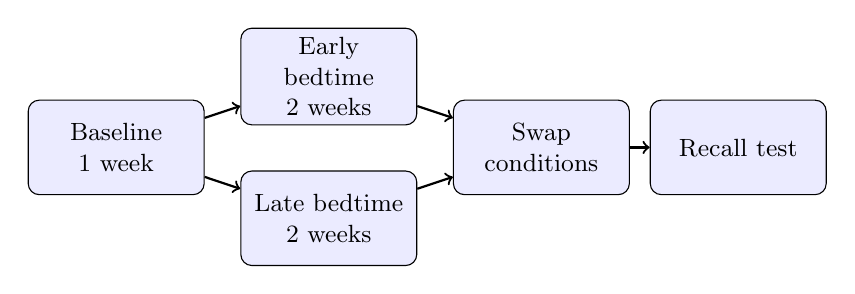
\begin{tikzpicture}[stage/.style={draw, rounded corners, fill=blue!8, text width=2cm, align=center, minimum height=1.2cm, font=\small}]
    \node[stage] (a) at (0,0) {Baseline\\1 week};
    \node[stage] (b) at (2.7,0.9) {Early bedtime\\2 weeks};
    \node[stage] (c) at (2.7,-0.9) {Late bedtime\\2 weeks};
    \node[stage] (d) at (5.4,0) {Swap\\conditions};
    \node[stage] (e) at (7.9,0) {Recall test};
    \draw[->, thick] (a) -- (b);
    \draw[->, thick] (a) -- (c);
    \draw[->, thick] (b) -- (d);
    \draw[->, thick] (c) -- (d);
    \draw[->, thick] (d) -- (e);
  \end{tikzpicture}
\end{frame}

\section{Results}
\begin{frame}{Key figure, redrawn}
  \begin{columns}[c]
    \begin{column}{0.5\textwidth}
      \centering
      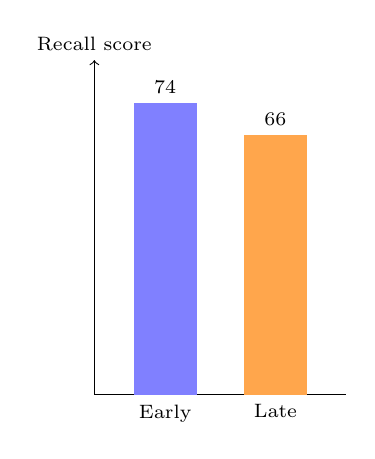
\begin{tikzpicture}[yscale=0.05]
        \draw[->] (0,0) -- (0,85) node[above, font=\scriptsize] {Recall score};
        \draw (0,0) -- (3.2,0);
        \fill[blue!50] (0.5,0) rectangle (1.3,74);
        \fill[orange!70] (1.9,0) rectangle (2.7,66);
        \node[below, font=\scriptsize] at (0.9,0) {Early};
        \node[below, font=\scriptsize] at (2.3,0) {Late};
        \node[above, font=\scriptsize] at (0.9,74) {74};
        \node[above, font=\scriptsize] at (2.3,66) {66};
      \end{tikzpicture}
    \end{column}
    \begin{column}{0.45\textwidth}
      \begin{block}{Our reading}
        The effect is clear, but error bars are not shown in the original figure.
      \end{block}
    \end{column}
  \end{columns}
\end{frame}

\section{Critique}
\begin{frame}{Strengths and weaknesses}
  \small
  \begin{tabular}{>{\raggedright\arraybackslash}p{0.44\linewidth}>{\raggedright\arraybackslash}p{0.44\linewidth}}
    \toprule
    \textbf{Strengths} & \textbf{Weaknesses} \\
    \midrule
    Crossover design controls for person differences & Small sample from one city \\
    Sleep measured with wrist devices, not diaries & Recall test only, no other memory types \\
    Pre registered hypotheses & Two week blocks may be too short \\
    \bottomrule
  \end{tabular}
\end{frame}

\begin{frame}{Discussion questions}
  \begin{enumerate}
    \item Would the effect hold for adults with fixed work hours?
    \item Is an 11\% change in recall meaningful in school settings?
    \item What follow up study would you design?
  \end{enumerate}
  \vspace{1em}
  \begin{alertblock}{Take home}
    Timing of sleep may matter, not only its length.
  \end{alertblock}
\end{frame}

\end{document}
